% !TeX root = ../main.tex

\chapter{阴影感知的光照表示研究}

本文第3章通过混合的几何表示以及MLP纹理,实现了能够对数字资产进行指定工作流分解的管线。
虽然实验能够证明管线的适用性,但是部分定量实验以及定性实验的结果显示,管线无法处理明显的阴影关系,
导致阴影中的几何形状和反射属性的分解效果较差。
以Metallic工作流为例,该工作流的分解结果如图\ref{fig:shadow_error}所示。
在\ref{fig:shadow_albedo}Albedo分解输出中,阴影被错误地处理为场景表面固有的颜色;
而在\ref{fig:shadow_mesh}网格体分解输出中,阴影影响了管线对几何结构的判断。
同样,在其它对NeRF进行光照分解的研究中\cite{Zhang_2021, Wu_2023},
也存在阴影处的数据无法正确处理的问题。

\begin{figure}[H]
  \centering
  % 这里可以控制图片宽度比例
  \begin{subfigure}[t]{0.3\textwidth}
    \centering
    \includegraphics[width=\linewidth]{ch4/compare_in_shadow/shadow_gt.png}
    \caption{GT}
    \label{fig:shadow_gt}
  \end{subfigure}
  \begin{subfigure}[t]{0.3\textwidth}
    \centering
    \includegraphics[width=\linewidth]{ch4/compare_in_shadow/shadow_albedo.png}
    \caption{Albedo分解输出}
    \label{fig:shadow_albedo}
  \end{subfigure}
  \begin{subfigure}[t]{0.3\textwidth}
    \centering
    \includegraphics[width=\linewidth]{ch4/compare_in_shadow/shadow_mesh.png}
    \caption{网格体分解输出}
    \label{fig:shadow_mesh}
  \end{subfigure}
  \caption{阴影处分解效果对比}
  \label{fig:shadow_error}
\end{figure}

结合第3章实验结果及其它研究,这种错误可能来自于光照表示方法的不足。因此本章将改进光照表示方法,
以解决这一问题。接下来,本章首先将详细分析现有光照技术的表示能力,随后介绍本文提出的新颖光照表示方法。

\section{光照表示能力分析}

2.3.1介绍了IBL技术,该技术通过预滤波处理将半球积分转化为查表运算,实现了复杂全局光照的实时近似计算。
然而这种近似必然伴随物理真实性的折损:
其核心假设将\eqref{eq:rendering_equation}渲染方程中的入射光照
$L_i\left(\mathbf{x},\omega_i\right)$简化为$L(\omega_i)$,
本质上忽略了着色点空间位置$\mathbf{x}$对入射光$L_i$的影响。
这种降维处理导致IBL难以表示阴影等局部光照变化,如图\ref{fig:shadow_n_refl}所示,
当着色点位于反射方向$\omega_i$相近的平面时,不同空间位置$\mathbf{x}$的着色点可能因为阴影而接收到完全不同的入射光$L_i$。
因此,在传统的即时渲染器中,IBL技术通常仅被用作阴影处的光照补充,而阴影之外的着色点则通过其它离散形式的光源进行计算。

\begin{figure}[htb]
  \centering
  % 这里可以控制图片宽度比例
  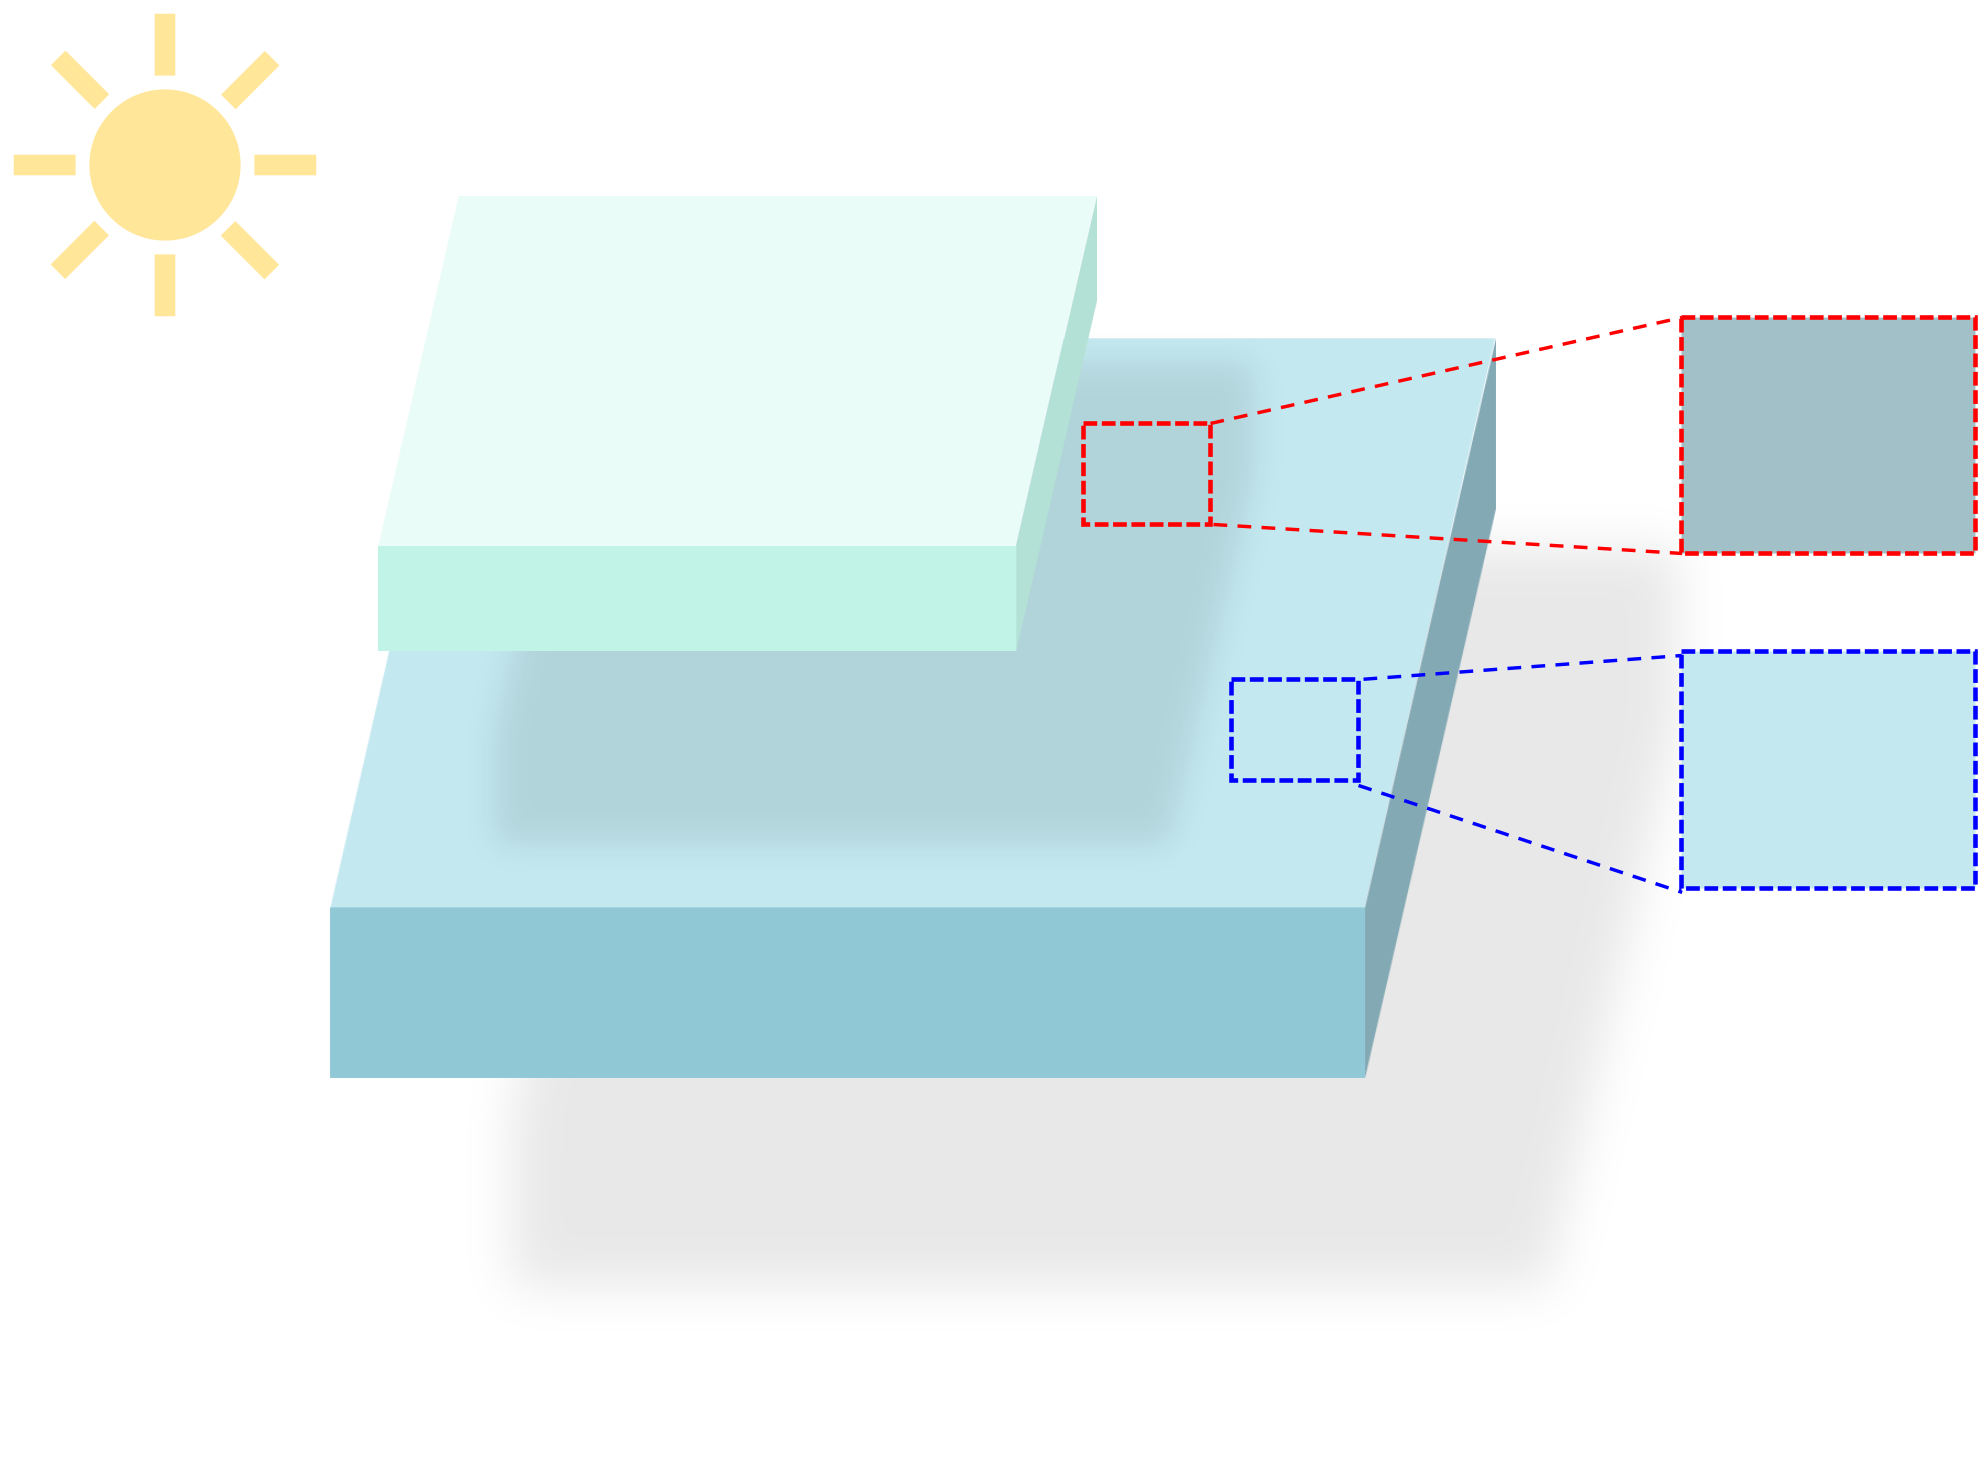
\includegraphics[width=0.8\linewidth]{ch4/shadow_n_refl.png}
  \caption{阴影对入射光照的影响}
  \label{fig:shadow_n_refl}
\end{figure}

为了改进这一点,本文考虑了上文所述的传统即时渲染中对IBL技术的应用方式,即仅将IBL作为完整光照的一部分补充,
用于增加阴影处的细节,记作环境光照$L_{env}$。而物体主要被直接光所照亮,记作$L_{direct}$。
本文中对直接光和环境光的分配可以由公式\eqref{eq:li_shadow}表示:
\begin{equation}
  \label{eq:li_shadow}
  L_i=\left(1-s\right)L_{\rm{direct}}+sL_{\rm{env}},
  \end{equation}

其中,$s$代表着色点处的阴影强度。该式反映出,直接光照的强度通常远高于环境光照,且只有直接光照能产生阴影,
而环境光照均匀地来自于一个球形的穹顶。因此,当着色点完全位于阴影之外时,环境光的贡献可以忽略,
直接光照主导;而当着色点进入阴影区域时,环境光的影响逐渐增加,成为主要的光照来源。
这种光照组合方式能够以较低的计算成本,显著提高阴影表示能力,同时几乎不增加优化的难度。
以上分析构成了本文创新的光照表示的基础,其并非对光照物理规律的完整数学描述,
而是将关键的物理原则嵌入到光照的组合方式中。这种策略在计算复杂度与光照表示能力之间取得了创新性平衡,
为后续的实现提供了清晰的框架。

\section{阴影调制模块与神经光照表示}

在上一节中,我们分析了IBL技术的局限性,并探讨了直接光和环境光的分配方式,
以进一步实现在较低的计算成本下增强光照表示能力的目标。基于以上分析,本文引入了神经光照表示方法,
以MLP为基础构建可学习的光照模型,从而扩展IBL在阴影场景中的适用性。

本节将介绍新颖的“阴影调制模块”,它能在神经网络的光照推理过程中引入对阴影的动态调控。
该模块不仅能捕捉局部阴影信息对光照分布的影响,还能与MLP主体紧密结合,从而在保持高效计算的同时,
大幅提升光照表示的准确度与逼真度。下面将详细阐述该模块的设计思路、实现细节以及它在神经光照表示框架中的作用。

\subsection{条件输入}

在机器学习中通常将基于上下文的处理称为条件:模型执行的计算会受到从辅助输入中提取的信息的制约或调节。
最简单的方法是将条件信息的表示与原有输入直接相连,将结果作为模型新的输入。该方法几乎不影响模型参数量,
但是条件信息会从输入层开始全部作用于后续的每一层。另一种方法是将条件信息与原输入相乘,条件信息可以对输入进行缩放,
以控制输入中哪些信息将进一步传递到后续的层。

Perez等人\cite{Perez_2018}将加法和乘积的方法结合,以仿射变换的形式将条件信息与输入结合,
称之为基于特征的线性变换(Feature-wise Linear Modulation,FiLM)。
仿射变换可以由公式\eqref{eq:film_affine}表示:
\begin{equation}
\label{eq:film_affine}
\varphi(x)=\gamma\cdot x+\beta
\end{equation}
其中,偏移量$\beta$和缩放系数$\gamma$被称为FiLM参数,仿射变换利用这些参数对输入$x$进行调制。

对于MLP来说,可以将特殊的FiLM层插入到模型中,以对该层的输入应用特征仿射变换。
FiLM参数(即偏移量$\beta$和缩放系数$\gamma$)由映射网络(Mappingnetwork)计算,
该网络利用条件信息$\mathbf{z}$作为输入,完成条件信息到FiLM参数的映射。
在这种设计下,虽然FiLM参数能够直接参与主网络的运算,但其实际为映射网络的输出结果,
因此FiLM参数不是传统意义上的具有固定权重的可学习参数,能够实现对主网络的调制。
FiLM层的计算方式如公式\eqref{eq:film_layer}所示,
\begin{equation}
\label{eq:film_layer}
\mathrm{FiLM}(\mathbf{x})=\gamma(\mathbf{z})\odot \mathbf{x}+\beta(\mathbf{z}).
\end{equation}
其中$\gamma(\mathbf{z})$和$\beta(\mathbf{z})$由映射网络计算,
$\odot$代表哈达玛乘积(Hadamard Product),对向量的各个分量之间逐个相乘。

本文则利用FiLM,将阴影视为条件输入至网络,利用FiLM调制阴影参数,以实现本文将阴影加入光照表示的目标。

\subsection{基于阴影调制模块的光照表示网络}

基于上述结构,本文设计了基于阴影调制模块的光照表示网络(Shadow-aware Neural Light,SaNL),其核心思想是将阴影系数$s$作为额外的标量参数调制到网络中。
当阴影系数为1时,在该模块的调制下,本文的网络将退化为一张环境光照贴图,其输出将全部为环境光照。
当阴影系数为0时,则使本文的网络输出为直接光照的光照强度及颜色。该网络的结构如\ref{fig:nl_main_cn}所示,
其接收入射光照的方向$\omega_i$作为输入,随后先调制阴影系数$s$,并在后续的层中逐步调制光照嵌入向量$\bf{z}^l$,
用以表示整张环境纹理。光照嵌入向量$\bf{z}^l$和阴影系数$s$的生成将在后文进一步介绍。

\begin{figure}[htb]
  \centering
  \includegraphics[width=0.6\linewidth]{ch4/nl_main_cn.png}
  \caption{光照表示网络结构图}
  \label{fig:nl_main_cn}
\end{figure}

对于映射网络,其结构如图\ref{fig:nl_main_cn}所示。该网络首先通过傅里叶编码将标量条件
输入映射到高维特征空间,从而提取出多频率的信息,增强了输入的表达能力。接着,转换后的特征被送入一个小型MLP,
该网络包含一个采用ELU激活函数的隐藏层,以捕捉输入数据的复杂特性;
随后,一个线性激活的全连接层进一步将特征映射到所需维度,并最终通过重塑操作生成参数对。

\begin{figure}[htb]
  \centering
  \includegraphics[width=0.6\linewidth]{ch4/mapping_net.png}
  \caption{映射网络结构图}
  \label{fig:nl_main_cn}
\end{figure}

最终,该光照表示网络将会构建类似“体积”纹理的光照表示,如图\ref{fig:nl_light_volume}所示,其根据阴影系数来对直接光照和环境光照进行插值,
实现了对两种光照的统一编码。

\begin{figure}[htb]
  \centering
  \includegraphics[width=0.6\linewidth]{ch4/sanl_light_show.png}
  \caption{网络光照关系示意图}
  \label{fig:nl_light_volume}
\end{figure}

\subsection{潜空间自动编码器}

对于上文提到的光照嵌入向量${\bf{z}}^l$,本文了参考Mark等人\cite{boss2021neural}的工作,通过自动编码器生成。
\ref{sec:auto_encoder}中介绍了自动编码器对于可微渲染的作用,Mark等人使用真实的环境纹理对自动编码器进行预训练,
该自动编码器能够将256$\times$256的环境纹理映射到128维向量,并使用多个损失函数约束潜空间,最终该自动编码器实现了
对具备真实感的光照潜空间,非常适合神经光照相关的任务。

该自动编码器通过四个损失函数的组合实现上述功能。首先是标准的重建损失$\mathcal{L}_{\mathcal{r}}$,可以通过以下公式定义:

\begin{equation}
  \label{eq:reconstruction_loss}
  \mathcal{L}_{\mathcal{r}}=\mathbb{C}_{E\sim\mathcal{D}_{\mathrm{light}}}\left[\|E-\mathcal{G}\left(\mathcal{E}(E)\right)\|_{\mathrm{Frobenius}}^2\right].
  \end{equation}
  其中$E$为编码器,$\mathcal{G}$为解码器,通过Frobenius范数保持像素级一致性。
  
  随后是循环一致损失$\mathcal{L}_{\mathcal{c}}$,该损失可以强制解码器的输出来自于编码器输入中的特征,其表达式为:
  \begin{equation}
  \label{eq:cycle_loss}
  \mathcal{L}_{\mathcal{c}}=\frac{1}{m}\sum_{n=1}^{m}\left|z_n'-\mathcal{E}\left(\mathcal{G}\left(z_n'\right)\right)\right|_{\Sigma^{-1}}^2.
  \end{equation}
  
  其次,为了使得潜空间向量$\mathcal{G}\left(z'\right)$生成的数据具备物理真实感,
  能够服从真实的光照分布,该自动编码器通过辨别器网络引入了对抗损失$\mathcal{L}_{\mathcal{a}}$:
  \begin{equation}
  \label{eq:adversarial_loss}
  \mathcal{L}_{\mathcal{a}}=\mathbb{C}_{z_a,z_b}\left[\|\mathcal{D}\left(\mathcal{G}\left(z'\right)\right)-1\|_2^2\right]+\mathbb{C}_E\left[\|\mathcal{D}\left(E\right)\|_2^2\right].
  \end{equation}
  这确保了插值的潜空间向量$\mathcal{G}\left(z'\right)$可以生成合理的数据,使得结果服从真实的光照分布,更具真实感。
  
  最后,该编码器使用曲率正则化$\mathcal{L}_{\mathcal{s}}$损失以确保流形局部平坦,
  避免生成的光照数据发生突变或空洞,其表达式为:
  \begin{equation}
  \label{eq:curvature_loss}
  \mathcal{L}_{\mathcal{s}}=\mathbb{C}_{\alpha\sim U\left(\mathbb{0},\mathbb{1}\right)}\left[\|J_{\mathcal{G}}\bigl(z(\alpha)\bigr)\cdot\frac{\partial z}{\partial\alpha}\|_{\mathrm{HS}}^2\right],
  \end{equation}
  其中$J_{\mathcal{G}}$为解码器的Jacobian矩阵,通过Hilbert-Schmidt范数惩罚路径曲率。
  
  最终的损失$\mathcal{L}$为上述四个损失的加权和,表达式为:
  \begin{equation}
  \label{eq:total_loss}
  \mathcal{L}=\mathcal{L}_{\mathcal{r}}+\lambda_1\mathcal{L}_{\mathcal{c}}+\lambda_2\mathcal{L}_{\mathcal{a}}+\lambda_3\mathcal{L}_{\mathcal{s}}.
\end{equation}

\section{数据集的获取}

由于本文希望SaNL能够学习到阴影与环境光照之间的关系,因此相较于其它的神经网络,
SaNL需要收集额外的数据集。根据前文的设计,SaNL需要入射光线方向$\omega_i$、阴影系数$s$、光照嵌入$z_l$作为输入数据,
以及入射光照$L_i$作为监督信号。本文通过渲染引擎收集了多组包含上述数据的合成数据集,下面介绍收集该数据集的方法及过程。

\section{入射光线方向数据}

在先前的研究中,入射光线方向$\omega_i$通常在训练时随机生成,不在数据集内提供。
本文考虑到入射光线方向与场景的几何形状直接相关,而IBL技术中,相似的几何形状可能在环境贴图中采样的区域相近,
因此本文选择根据网格体来收集真实的场景几何形状。为了增强数据集的多样性,在选择网格体时应充分考虑包括不同的几何结构。
同时,为了方便收集阴影系数数据,网格体也应有丰富的自遮挡。

本文选取的8个网格体如图\ref{fig:data_mesh}所示。这些网格体形状各异,如Sofa、Car等网格体具有细微尖锐的高频细节,
Teapot、Statue有平滑圆润的表面,而Beach、Girl的几何结构则能生成充分的自阴影。

\begin{figure}[htbp]
  \centering
  \renewcommand{\arraystretch}{1} % 调整表格行距
  \setlength{\tabcolsep}{3pt} % 调整列间距

  \begin{tabular}{c c c c}
      \subfloat{\includegraphics[width=0.22\textwidth]{ch4/sanl_data_mesh/beach.png}} &
      \subfloat{\includegraphics[width=0.22\textwidth]{ch4/sanl_data_mesh/Girl.png}} &
      \subfloat{\includegraphics[width=0.22\textwidth]{ch4/sanl_data_mesh/chair.png}} &
      \subfloat{\includegraphics[width=0.22\textwidth]{ch4/sanl_data_mesh/Car.png}} \\
      Beach & Girl & Sofa & Car\\

      \subfloat{\includegraphics[width=0.22\textwidth]{ch4/sanl_data_mesh/Rabbit.png}} &
      \subfloat{\includegraphics[width=0.22\textwidth]{ch4/sanl_data_mesh/Skull.png}} &
      \subfloat{\includegraphics[width=0.22\textwidth]{ch4/sanl_data_mesh/Teapot.png}} &
      \subfloat{\includegraphics[width=0.22\textwidth]{ch4/sanl_data_mesh/Statue.png}} \\
      Rabbit & Skull & Teapot & Statue\\
  \end{tabular}

  \caption{构成数据集的网格体}
  \label{fig:data_mesh}
\end{figure}

\subsection{光照与阴影数据}

入射光照数据$L_i$作为SaNL的监督信号,需要充分考虑直接光照和环境光照的关系。对于环境光照,
本文使用了500张高质量的HDR立方体纹理作为环境光照的数据来源,这些立方体纹理将以IBL技术向场景内投射光照,
同时,为了获得更加多样的环境光照数据,这些立方体纹理会围绕$Z$轴随机旋转,尽可能地记录纹理中不同区域的光照。

直接光照部分,本文使用单盏平行光模拟,随机生成光照方向。为了使直接光照更符合真实情况,
直接光照的仰角随机范围为[15, 85]之间,方位角范围为[0, 360]之间。同时,为了增加网络对不同颜色的直接光照的泛化性,
本文使用色温描述直接光照颜色,随机范围为[5000, 10000]开尔文。阴影数据$s$也同样由该盏直接光照在网格体上照射产生。
直接光照和环境光照将按照公式\eqref{eq:li_shadow}进行插值,并输出为监督信号$L_i$。

对于光照嵌入向量$z_l$,需要一张环境纹理$I$作为自动编码器进行计算,因此本文将上述环境光照和直接光照烘焙至
一张新的HDR立方体贴图,分辨率为$128\times128\times6$。这种烘焙的策略能使得光照嵌入向量$z_l$不仅保留了环境光照的信息,
还加入了直接光照的亮度、色温、方向等信息。烘焙前后的对比如图所示。

\begin{figure}[H]
  \centering
  % 这里可以控制图片宽度比例
  \begin{subfigure}[t]{0.45\textwidth}
    \centering
    \includegraphics[width=\linewidth]{ch4/data_set/before.png}
    \caption{烘焙前}
  \end{subfigure}
  \begin{subfigure}[t]{0.45\textwidth}
    \centering
    \includegraphics[width=\linewidth]{ch4/data_set/after.png}
    \caption{烘焙后}
  \end{subfigure}
  \caption{环境光照与直接光照烘焙}
  \label{fig:light_baking}
\end{figure}

最终,完整的数据收集过程如图\ref{fig:full_pipe}所示。

\begin{figure}[htb]
  \centering
  % 这里可以控制图片宽度比例
  \includegraphics[width=0.6\linewidth]{ch4/data_set/full_pipe.png}
  \caption{数据集完整收集流程}
  \label{fig:full_pipe}
\end{figure}

\section{基于SaNL的解耦管线实现}

前文中,我们通过实验结果分析了管线无法处理阴影的原因,随后根据问题设计了SaNL,并收集了对应的数据进行训练。
本节将使用SaNL作为光照表示技术,实现数字资产解耦管线,以提升管线的分解效果。

\subsection{阴影系数}

由于本文第三章所设计的管线并不支持对阴影的建模,而SaNL的输入依赖于直接光照所产生的投影作为阴影系数$s$,
因此有必要对阴影建模进行额外的实现和处理。现有的部分NeRF分解管线支持阴影的计算,
但部分工作需要已知光源信息才能对直接光照的投影进行计算,而另外一些工作则依赖额外的光线追踪阶段。
这些方法通常是为了适用于复杂的光照条件,由于本文的研究目标是对数字资产的合成数据进行分解,
输入数据的光照环境在实验中更具有可控性,相比于真实数据中实时变化的光照条件,这为阴影系数的建模提供了有利的条件。

因此,在每张输入图像的光照条件不变的前提下,阴影系数可以被视为覆盖场景各处的贴图,
这一方法类似于传统渲染技术中常见的烘焙光照贴图技术(Baked Light Map)。
烘焙光照贴图的基本原理是通过对场景的几何结构和特定的光照条件进行预计算,将光照、阴影信息存储在一张纹理图中,
其中每个像素值表示相应区域所接受的入射光照强度,如图\ref{fig:baked_light_map}所示。这种方法能够有效减少实时渲染中的计算负担,
因为阴影信息已经在渲染前通过烘焙过程完成了计算。

\begin{figure}[H]
  \centering
  % 这里可以控制图片宽度比例
  \begin{subfigure}[t]{0.45\textwidth}
    \centering
    \includegraphics[height=6cm,keepaspectratio]{ch4/baked_light_map/scene.png}
    \caption{复杂光照的场景}
  \end{subfigure}
  \hspace{0.05\textwidth} % 添加间隔
  \begin{subfigure}[t]{0.45\textwidth}
    \centering
    \includegraphics[height=6cm,keepaspectratio]{ch4/baked_light_map/light map.png}
    \caption{光照和阴影的烘焙结果}
  \end{subfigure}
  \caption{烘焙光照贴图技术}
  \label{fig:baked_light_map}
\end{figure}

本文采用了类似的策略,将阴影系数表示为一张灰度贴图,利用\ref{sec:mlp_texture}中所述的MLP纹理来进行估计。
另外,考虑到在本课题的设置中,光照网络已经完成了一次阴影的计算,因此在最终的着色过程中,
不再需要重复计算阴影。阴影的计算及输出如图\ref{fig:shadow_mapping}所示,阴影区域能够得到正确的区分。

\begin{figure}[H]
  \centering
  % 这里可以控制图片宽度比例
  \begin{subfigure}[c]{0.27\textwidth}
    \centering
    \includegraphics[width=\linewidth]{ch4/shadow/gt.png}
    \caption{原场景}
  \end{subfigure}
  \hspace{0.05\textwidth} % 添加间隔
  \begin{subfigure}[c]{0.27\textwidth}
    \centering
    \includegraphics[width=\linewidth]{ch4/shadow/shadow.png}
    \caption{场景阴影系数}
  \end{subfigure}
  \hspace{0.05\textwidth} % 添加间隔
  \begin{subfigure}[c]{0.27\textwidth}
    \centering
    \includegraphics[width=\linewidth]{ch4/shadow/shadow_texture.png}
    \caption{阴影系数纹理}
  \end{subfigure}
  \caption{阴影系数的计算}
  \label{fig:shadow_mapping}
\end{figure}


\section{整体管线结构}

\section{实验结果与分析}

在前四节中,本文通过新颖的阴影调制模块实现了SaNL,能够在表示光照的同时将阴影与直接光照的信息进行建模。
随后,本文将SaNL加入第三章的数字资产管线,以提升对网格体和表面属性分解的效果。在这一节中,
本文将首先对SaNL进行全面的实验,以验证其对光照的表示能力。随后,
本文将带有SaNL的数字资产解耦管线与相关研究进行横向的定量定性对比,以显示本文方法的优越性。
最后,本节还对管线进行了定量定性的消融实验,进一步说明了本文相关方法的工作原理和有效性。

\subsection{网络光照输出结果}
在本节中,本文通过实验展示了光照网络的输出效果。实验环境设置为几何形状和阴影已知,监督信号为真实的带阴影光照效果。
本实验展示了光照网络在不同的环境贴图下的输出结果,如图\ref{fig:SaNL_result}所示。

\begin{figure}[htbp]
  \centering
  \renewcommand{\arraystretch}{1}
  \setlength{\tabcolsep}{3pt}

  \begin{tabular}{c @{\hspace{10pt}} c c @{\hspace{10pt}} c c @{\hspace{10pt}} c c @{\hspace{10pt}} c c} 
      & \multicolumn{2}{c}{Peak} 
      & \multicolumn{2}{c}{Forest} 
      & \multicolumn{2}{c}{Sunset} 
      & \multicolumn{2}{c}{Ginko} \\ [2mm]

      & \multicolumn{2}{c}{\includegraphics[width=0.12\textwidth]{ch4/sanl_full_result/Peak.png}} 
      & \multicolumn{2}{c}{\includegraphics[width=0.12\textwidth]{ch4/sanl_full_result/Forest.png}}
      & \multicolumn{2}{c}{\includegraphics[width=0.12\textwidth]{ch4/sanl_full_result/Sunset.png}}
      & \multicolumn{2}{c}{\includegraphics[width=0.12\textwidth]{ch4/sanl_full_result/Ginko.png}} \\ [1mm]

      \raisebox{1.8\height}{\rotatebox[origin=c]{90}{Sofa}} & 
      \subfloat{\includegraphics[width=0.1\textwidth]{ch4/sanl_full_result/Sofa/Peak_GT.png}} &
      \subfloat{\includegraphics[width=0.1\textwidth]{ch4/sanl_full_result/Sofa/Peak_Ours.png}} &
      \subfloat{\includegraphics[width=0.1\textwidth]{ch4/sanl_full_result/Sofa/Forest_GT.png}} &
      \subfloat{\includegraphics[width=0.1\textwidth]{ch4/sanl_full_result/Sofa/Forest_Ours.png}} &
      \subfloat{\includegraphics[width=0.1\textwidth]{ch4/sanl_full_result/Sofa/Sunset_GT.png}} &
      \subfloat{\includegraphics[width=0.1\textwidth]{ch4/sanl_full_result/Sofa/Sunset_Ours.png}} &
      \subfloat{\includegraphics[width=0.1\textwidth]{ch4/sanl_full_result/Sofa/Ginko_GT.png}} &
      \subfloat{\includegraphics[width=0.1\textwidth]{ch4/sanl_full_result/Sofa/Ginko_Ours.png}} \\

      \raisebox{0.9\height}{\rotatebox[origin=c]{90}{Umbrella}} & 
      \subfloat{\includegraphics[width=0.1\textwidth]{ch4/sanl_full_result/Umbrella/Peak_GT.png}} &
      \subfloat{\includegraphics[width=0.1\textwidth]{ch4/sanl_full_result/Umbrella/Peak_Ours.png}} &
      \subfloat{\includegraphics[width=0.1\textwidth]{ch4/sanl_full_result/Umbrella/Forest_GT.png}} &
      \subfloat{\includegraphics[width=0.1\textwidth]{ch4/sanl_full_result/Umbrella/Forest_Ours.png}} &
      \subfloat{\includegraphics[width=0.1\textwidth]{ch4/sanl_full_result/Umbrella/Sunset_GT.png}} &
      \subfloat{\includegraphics[width=0.1\textwidth]{ch4/sanl_full_result/Umbrella/Sunset_Ours.png}} &
      \subfloat{\includegraphics[width=0.1\textwidth]{ch4/sanl_full_result/Umbrella/Ginko_GT.png}} &
      \subfloat{\includegraphics[width=0.1\textwidth]{ch4/sanl_full_result/Umbrella/Ginko_Ours.png}} \\

      \raisebox{1.5\height}{\rotatebox[origin=c]{90}{Skull}} & 
      \subfloat{\includegraphics[width=0.1\textwidth]{ch4/sanl_full_result/Skull/Peak_GT.png}} &
      \subfloat{\includegraphics[width=0.1\textwidth]{ch4/sanl_full_result/Skull/Peak_Ours.png}} &
      \subfloat{\includegraphics[width=0.1\textwidth]{ch4/sanl_full_result/Skull/Forest_GT.png}} &
      \subfloat{\includegraphics[width=0.1\textwidth]{ch4/sanl_full_result/Skull/Forest_Ours.png}} &
      \subfloat{\includegraphics[width=0.1\textwidth]{ch4/sanl_full_result/Skull/Sunset_GT.png}} &
      \subfloat{\includegraphics[width=0.1\textwidth]{ch4/sanl_full_result/Skull/Sunset_Ours.png}} &
      \subfloat{\includegraphics[width=0.1\textwidth]{ch4/sanl_full_result/Skull/Ginko_GT.png}} &
      \subfloat{\includegraphics[width=0.1\textwidth]{ch4/sanl_full_result/Skull/Ginko_Ours.png}} \\

      \raisebox{1.8\height}{\rotatebox[origin=c]{90}{Girl}} & 
      \subfloat{\includegraphics[width=0.1\textwidth]{ch4/sanl_full_result/Girl/Peak_GT.png}} &
      \subfloat{\includegraphics[width=0.1\textwidth]{ch4/sanl_full_result/Girl/Peak_Ours.png}} &
      \subfloat{\includegraphics[width=0.1\textwidth]{ch4/sanl_full_result/Girl/Forest_GT.png}} &
      \subfloat{\includegraphics[width=0.1\textwidth]{ch4/sanl_full_result/Girl/Forest_Ours.png}} &
      \subfloat{\includegraphics[width=0.1\textwidth]{ch4/sanl_full_result/Girl/Sunset_GT.png}} &
      \subfloat{\includegraphics[width=0.1\textwidth]{ch4/sanl_full_result/Girl/Sunset_Ours.png}} &
      \subfloat{\includegraphics[width=0.1\textwidth]{ch4/sanl_full_result/Girl/Ginko_GT.png}} &
      \subfloat{\includegraphics[width=0.1\textwidth]{ch4/sanl_full_result/Girl/Ginko_Ours.png}} \\ [1mm]

      & GT & Ours & GT & Ours & GT & Ours & GT & Ours \\
  \end{tabular}

  \caption{SaNL输出结果}
  \label{fig:SaNL_result}
\end{figure}

图\ref{fig:sanl_single_compare}则展示了本文网络的放大对比,可以看到SaNL在阴影处能够较好地还原环境贴图的细节,
实现了按照阴影系数对直接光照和环境光照进行区分的目标,并且在直接光照部分保持了原输入的色温及亮度。

\begin{figure}[H]
  \centering
  % 这里可以控制图片宽度比例
  \begin{subfigure}[c]{0.23\textwidth}
    \centering
    \includegraphics[height=5cm,keepaspectratio]{ch4/sanl_single_compare/Girl/GT.png}
    \caption{GT}
  \end{subfigure}
  \begin{subfigure}[c]{0.23\textwidth}
    \centering
    \includegraphics[height=5cm,keepaspectratio]{ch4/sanl_single_compare/Girl/Ours.png}
    \caption{Ours}
  \end{subfigure}
  \hspace{0.05\textwidth} % 添加间隔
  \begin{subfigure}[c]{0.23\textwidth}
    \centering
    \includegraphics[height=5cm,keepaspectratio]{ch4/sanl_single_compare/Girl/Env.png}
    \caption{环境贴图局部}
  \end{subfigure}
  \caption{局部放大对比}
  \label{fig:sanl_single_compare}
\end{figure}

图\ref{fig:sanl_single_compare_failure}展示了SaNL的失败案例,在这张环境纹理中,亮度和饱和度差异较低,
同时考虑到输入网格体的椅背部分反射角度近似,但是部分位于阴影中、部分暴露于直接光照之下,
因此网络难以区分直接光照和环境光照,导致高频细节还原失败,同时阴影处着色不正确。

\begin{figure}[H]
  \centering
  % 这里可以控制图片宽度比例
  \begin{subfigure}[c]{0.23\textwidth}
    \centering
    \includegraphics[height=5cm,keepaspectratio]{ch4/sanl_single_compare/Chair/GT.png}
    \caption{GT}
  \end{subfigure}
  \begin{subfigure}[c]{0.23\textwidth}
    \centering
    \includegraphics[height=5cm,keepaspectratio]{ch4/sanl_single_compare/Chair/Ours.png}
    \caption{Ours}
  \end{subfigure}
  \hspace{0.05\textwidth} % 添加间隔
  \begin{subfigure}[c]{0.23\textwidth}
    \centering
    \includegraphics[height=5cm,keepaspectratio]{ch4/sanl_single_compare/Chair/Env.png}
    \caption{环境贴图局部}
  \end{subfigure}
  \caption{失败案例}
  \label{fig:sanl_single_compare_failure}
\end{figure}

\subsection{完整管线实验}

本节将该光照网络接入至本文第三章所设计的管线,并横向对比了与本文类似的工作进行定量定性的实验。
图\ref{fig:full_rendering_result}展示了NeRD\cite{Boss_2021}、nvdiffremc\cite{10.5555/3600270.3601931}与本文管线效果的对比,
尤其是在阴影覆盖的区域中,本文能够较好地还原场景表面细节。比如Lego场景中,
红色线框和蓝色线框中的细节均能成功还原。

\begin{figure}[htbp]
  \centering
  \renewcommand{\arraystretch}{1} % 调整表格行距
  \setlength{\tabcolsep}{3pt} % 调整列间距

  \begin{tabular}{c c c c c} 
      & NeRD\cite{Boss_2021} & nvdiffremc\cite{10.5555/3600270.3601931} & Ours & GT\\

      \raisebox{2.7\height}{\rotatebox[origin=c]{90}{Lego}} & % 关键修改
      \subfloat{\includegraphics[width=0.22\textwidth]{ch4/full_pipe/lego/nerd.png}} &
      \subfloat{\includegraphics[width=0.22\textwidth]{ch4/full_pipe/lego/nvdiffrecmc.png}} &
      \subfloat{\includegraphics[width=0.22\textwidth]{ch4/full_pipe/lego/ours.png}} &
      \subfloat{\includegraphics[width=0.22\textwidth]{ch4/full_pipe/lego/GT_tagged.png}} \\

      \raisebox{2.2\height}{\rotatebox[origin=c]{90}{Hotdog}} & % 关键修改
      \subfloat{\includegraphics[width=0.22\textwidth]{ch4/full_pipe/Hotdog/nerd.png}} &
      \subfloat{\includegraphics[width=0.22\textwidth]{ch4/full_pipe/Hotdog/nvdiffrecmc.png}} &
      \subfloat{\includegraphics[width=0.22\textwidth]{ch4/full_pipe/Hotdog/ours.png}} &
      \subfloat{\includegraphics[width=0.22\textwidth]{ch4/full_pipe/Hotdog/GT_tagged.png}} \\

      \raisebox{1.7\height}{\rotatebox[origin=c]{90}{Materials}} & % 关键修改
      \subfloat{\includegraphics[width=0.22\textwidth]{ch4/full_pipe/Materials/nerd.png}} &
      \subfloat{\includegraphics[width=0.22\textwidth]{ch4/full_pipe/Materials/nvdiffrecmc.png}} &
      \subfloat{\includegraphics[width=0.22\textwidth]{ch4/full_pipe/Materials/ours.png}} &
      \subfloat{\includegraphics[width=0.22\textwidth]{ch4/full_pipe/Materials/GT_tagged.png}} \\

      \raisebox{3.2\height}{\rotatebox[origin=c]{90}{Mic}} & % 关键修改
      \subfloat{\includegraphics[width=0.22\textwidth]{ch4/full_pipe/Mic/nerd.png}} &
      \subfloat{\includegraphics[width=0.22\textwidth]{ch4/full_pipe/Mic/nvdiffrecmc.png}} &
      \subfloat{\includegraphics[width=0.22\textwidth]{ch4/full_pipe/Mic/ours.png}} &
      \subfloat{\includegraphics[width=0.22\textwidth]{ch4/full_pipe/Mic/GT_tagged.png}} \\

  \end{tabular}

  \caption{渲染结果横向比较}
  \label{fig:full_rendering_result}
\end{figure}

表\ref{tab:dataset_comparison}展示了本文方法与其它方法的定量比较结果。其中,NeRF-Synthetic数据集、NeRFactor数据集为合成数据,
NeRD数据集则包含则仅使用其中的三个合成场景。根据实验结果,本文管线在以上数据集中均取得了最优的成绩,可以证明本文方法的优越性。

\begin{table}[h]
  \centering
  \caption{渲染结果定量比较}
  \begin{tabular}{l ccc ccc ccc}
      \toprule
      & \multicolumn{3}{c}{NeRF-Synthetic} & \multicolumn{3}{c}{NeRD Dataset} & \multicolumn{3}{c}{DTU Dataset} \\
      \cmidrule(lr){2-4} \cmidrule(lr){5-7} \cmidrule(lr){8-10}
      & PSNR$\uparrow$ & LPIPS$\downarrow$ & SSIM$\uparrow$ & PSNR$\uparrow$ & LPIPS$\downarrow$ & SSIM$\uparrow$ & PSNR$\uparrow$ & LPIPS$\downarrow$ & SSIM$\uparrow$ \\
      \midrule
      NeRD & & & & & & & & & \\
      nvdiffrecmc & 26.35 & 0.097 & 0.910 & 25.58 & 0.081 & 0.918 & 25.78 & 0.088 & 0.912 \\
      \textbf{Ours} & \textbf{29.03} & \textbf{0.053} & \textbf{0.948} & \textbf{25.70} & \textbf{0.091} & \textbf{0.921} & \textbf{29.42} & \textbf{0.053} & \textbf{0.947} \\
      \bottomrule
  \end{tabular}
  \label{tab:dataset_comparison}
\end{table}

图\ref{fig:rendering_detail_compare}展示了管线导出的网格体效果对比。本文的管线不仅在阴影处取得了更好的重建效果,
同时也能够较为准确地对履带等阴影处的细节进行重建。

\begin{figure}[H]
  \centering
  % 这里可以控制图片宽度比例
  \begin{subfigure}[c]{0.32\textwidth}
    \centering
    \includegraphics[height=5.1cm,keepaspectratio]{ch4/rendering_detail/ours_full.png}
    \caption{Our Results}
  \end{subfigure}
  \begin{subfigure}[c]{0.16\textwidth}
    \centering
    \includegraphics[height=5.1cm,keepaspectratio]{ch4/rendering_detail/nerd.png}
    \caption{NeRD}
  \end{subfigure}
  \hspace{0.1mm}
  \begin{subfigure}[c]{0.16\textwidth}
    \centering
    \includegraphics[height=5.1cm,keepaspectratio]{ch4/rendering_detail/nvdiffrecmc.png}
    \caption{nvdiffremc}
  \end{subfigure}
  \hspace{0.1mm}
  \begin{subfigure}[c]{0.16\textwidth}
    \centering
    \includegraphics[height=5.1cm,keepaspectratio]{ch4/rendering_detail/ours.png}
    \caption{Ours}
  \end{subfigure}
  \hspace{0.1mm}
  \begin{subfigure}[c]{0.16\textwidth}
    \centering
    \includegraphics[height=5.1cm,keepaspectratio]{ch4/rendering_detail/GT.png}
    \caption{GT}
  \end{subfigure}
  \caption{渲染结果细节对比}
  \label{fig:rendering_detail_compare}
\end{figure}

图\ref{fig:mesh_export_compare}展示了管线导出的网格体效果对比。NeRD无法直接导出网格体,而nvdiffrec产生了较多破面,并且在阴影处错误估计了几何形状。
本文的管线不仅在阴影处取得了更好的重建效果,同时也能够较为准确地对履带等阴影处的细节进行重建。

\begin{figure}[H]
  \centering
  % 这里可以控制图片宽度比例
  \begin{subfigure}[c]{0.32\textwidth}
    \centering
    \includegraphics[height=5.1cm,keepaspectratio]{ch4/mesh_detail/ours_result.png}
    \caption{Our Results}
  \end{subfigure}
  \begin{subfigure}[c]{0.16\textwidth}
    \centering
    \includegraphics[height=5.1cm,keepaspectratio]{ch4/mesh_detail/nerd.png}
    \caption{NeRD}
  \end{subfigure}
  \hspace{0.1mm}
  \begin{subfigure}[c]{0.16\textwidth}
    \centering
    \includegraphics[height=5.1cm,keepaspectratio]{ch4/mesh_detail/nvdiffrecmc.png}
    \caption{nvdiffremc}
  \end{subfigure}
  \hspace{0.1mm}
  \begin{subfigure}[c]{0.16\textwidth}
    \centering
    \includegraphics[height=5.1cm,keepaspectratio]{ch4/mesh_detail/ours.png}
    \caption{Ours}
  \end{subfigure}
  \hspace{0.1mm}
  \begin{subfigure}[c]{0.16\textwidth}
    \centering
    \includegraphics[height=5.1cm,keepaspectratio]{ch4/mesh_detail/GT.png}
    \caption{GT}
  \end{subfigure}
  \caption{网格体导出效果对比}
  \label{fig:mesh_export_compare}
\end{figure}

\subsection{SaNL消融实验}

本节将通过消融实验,证明SaNL在数字资产解耦任务中的有效性。图\ref{fig:}展示了本文管线使用及不使用SaNL时,
在Metallic工作流中对Albedo分解效果的对比。可以清晰地看到,在阴影处的Albedo可以准确地还原物体原本的颜色,
准确地区分出了浅色物体和深色物体,并且有准确的白平衡。

\begin{figure}[H]
  \centering
  % 这里可以控制图片宽度比例
  \begin{subfigure}[c]{0.47\textwidth}
    \centering
    \includegraphics[width=\textwidth]{ch4/sanl_ablation/albedo/ours.png}
    \caption{Ours}
  \end{subfigure}
  \begin{subfigure}[c]{0.47\textwidth}
    \centering
    \includegraphics[width=\textwidth]{ch4/sanl_ablation/albedo/wo.png}
    \caption{w/o SaNL}
  \end{subfigure}
  \caption{Albedo输出消融实验结果}
  \label{fig:albedo_ablation}
\end{figure}

图\ref{fig:mesh_ablation}为管线网格体输出的输出结果。在阴影中的盘子得到了准确平滑的还原,
而不使用SaNL时则将盘子上的阴影错误地处理为了几何结构,导致重建结果不佳。

\begin{figure}[H]
  \centering
  % 这里可以控制图片宽度比例
  \begin{subfigure}[c]{0.47\textwidth}
    \centering
    \includegraphics[width=\textwidth]{ch4/sanl_ablation/mesh/ours.png}
    \caption{Ours}
  \end{subfigure}
  \begin{subfigure}[c]{0.47\textwidth}
    \centering
    \includegraphics[width=\textwidth]{ch4/sanl_ablation/mesh/wo.png}
    \caption{w/o SaNL}
  \end{subfigure}
  \caption{网格体输出消融实验结果}
  \label{fig:mesh_ablation}
\end{figure}



